\documentclass[11pt]{report}
\usepackage{geometry}                % See geometry.pdf to learn the layout options. There are lots.
\geometry{letterpaper}                   % ... or a4paper or a5paper or ... 
%\geometry{landscape}                % Activate for for rotated page geometry
%\usepackage[parfill]{parskip}    % Activate to begin paragraphs with an empty line rather than an indent
\usepackage{graphicx}
\usepackage{amssymb}
\usepackage{epstopdf}
\DeclareGraphicsRule{.tif}{png}{.png}{`convert #1 `dirname #1`/`basename #1 .tif`.png}

\title{AIS Storage user guide}
\author{Xavier Tordoir}
%\date{}                                           % Activate to display a given date or no date


\begin{document}
\maketitle
\tableofcontents
\part{Prerequisites}
\chapter{Definitions and concepts}
The AIS storage system is a cloud based storage system. As such, storage operations are performed by HTTP requests exclusively, either through the web application or the REST API, the latter operation being wrapped in java and python libraries. The system is very similar to the Amazon S3 or Google Storage products. The main features differentiating these products from our solution is that the physical storage is provided by third parties and not exclusively by us.
\section{bucket}
A Bucket is a container for files and objects. The user can consider a bucket as a kind of virtual disk or workspace. Buckets cannot be nested, they are always the root of a set of data to be organized within the bucket. Sharing data with collaborators and customers is configured at the bucket level, all objects within a bucket share the same access rules. The user can so consider a bucket as a single project allowing to grant access on its content to other selected users.
\section{bucket metadata}
Bucket Metadata are sets of key-value pairs associated with a bucket. These metadata allow the owner of a bucket to configure the behaviour of the bucket with respect to data storage (see �...), and to add some general information about the bucket.
\section{object}
Objects are the elements contained in a bucket, no object can exist outside of a bucket.  All objects have a \emph{key} with is a text uniquely identifying the object within the bucket. In a simple usage scenario, the \emph{key} is the path of a file or directory within the bucket.\\
An object is actually a pointer to a unit of data. This object can point to a file, a directory or any other type of data that can be stored in the form of object metadata. 
\section{object metadata}
Metadata in the form of key-value pairs can be associated with objects. This mechanism is used for example to identify an object as a file on a physical storage device. These metadata allow to configure the behaviour of an object (for example a file can be downloaded), or for the user to add some general information about the object.
\section{store}
While the list of objects stored in buckets as well as metadata are maintained in a database, files are stored on physical disks. The system is able to access these physical files through the concept of stores. A store is an ssh connection to a server providing storage space. This connection is a username, a server address (IP or dns) and a root directory under which all data are stored.
\begin{figure}[htbp]
   \centering
   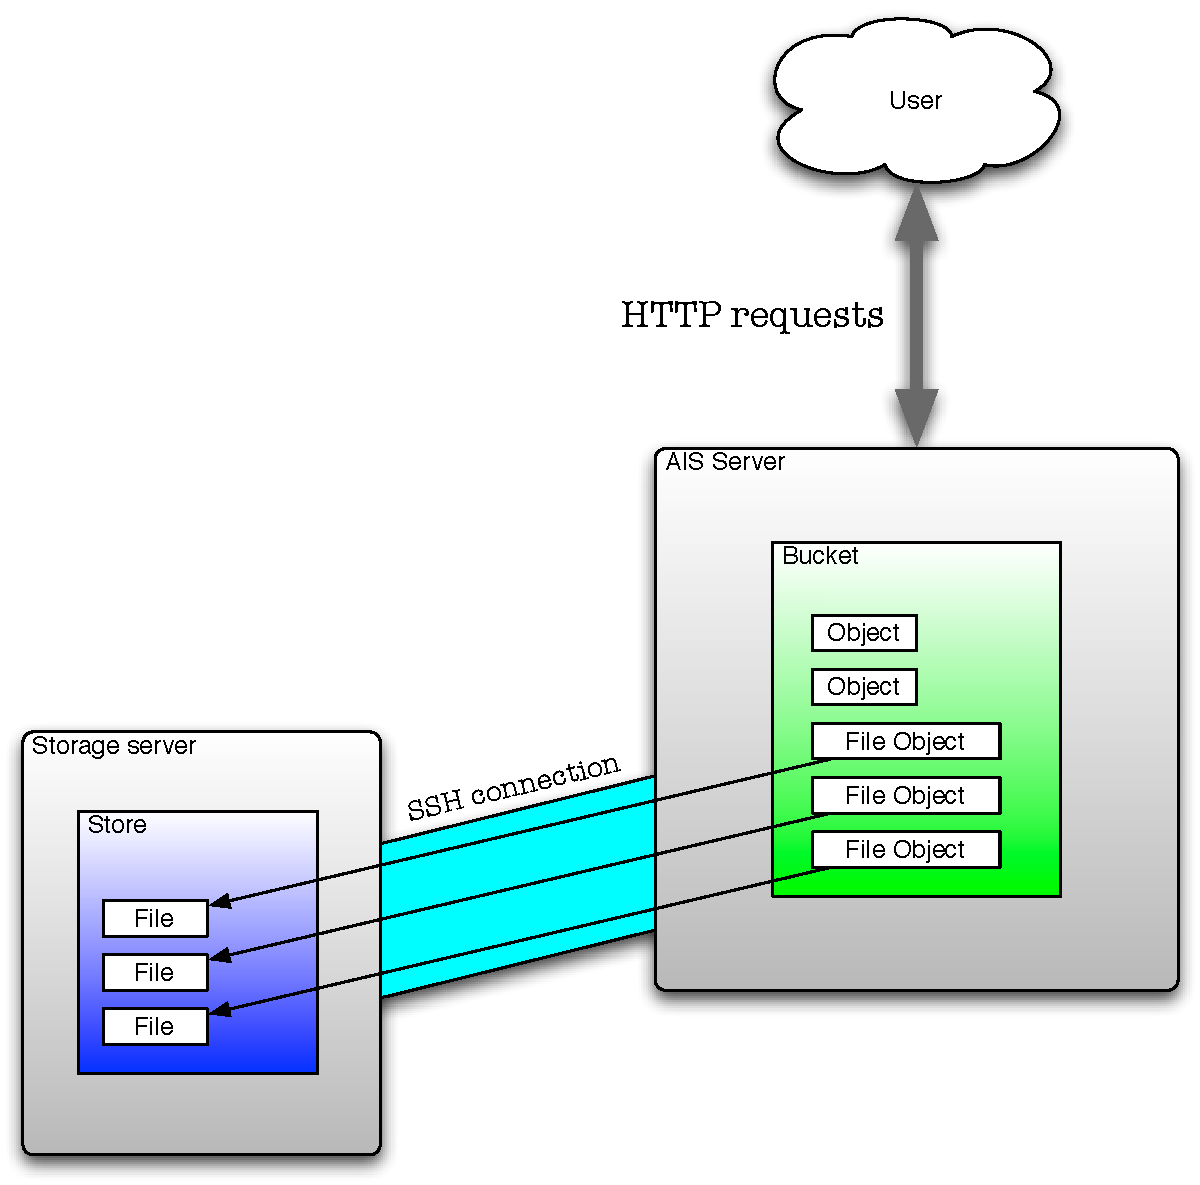
\includegraphics[width=1.0\linewidth]{store-bucket-object.pdf} % requires the graphicx package
   \caption{Relationship between a store, a bucket and objects. The user interacts with the AIS server through secured HTTP requests. The AIS server manages buckets and objects. File objects point to files stored in a storage server. The AIS server serves those file by connecting through an SSH connection (the store) to the storage server.}
   \label{fig:store-bucket-object}
\end{figure}

\part{User guide: web interface}
\chapter{Store management}
The use of the storage system relies on a database used to store the buckets and objects definitions and metadata on one side and on a number of \emph{store} to store the files on the other side (see figure~\ref{fig:store-bucket-object}). The database is provided by the AIS storage middleware, while the stores are dynamically plugged on the system and access is granted to users. So store management is the basics to be able to manage files in the system.\\
Most users will not actively manage stores, but will simply use them, as storage back-end for their files, in a transparent way. So this chapter is intended for physical storage providers or users wanting to know more about the file storage details.
\section{Stores general navigation}
From the \emph{Storage} tab, the store panel is available and features the list of stores the user has access to. Read only stores provide a button to request write access, and if administration rights are granted, an access to the rights management page is also available.\\
It is from that view that new stores can be created as well (see figure~\ref{fig:storesview}).
\begin{figure}[htbp]
   \centering
   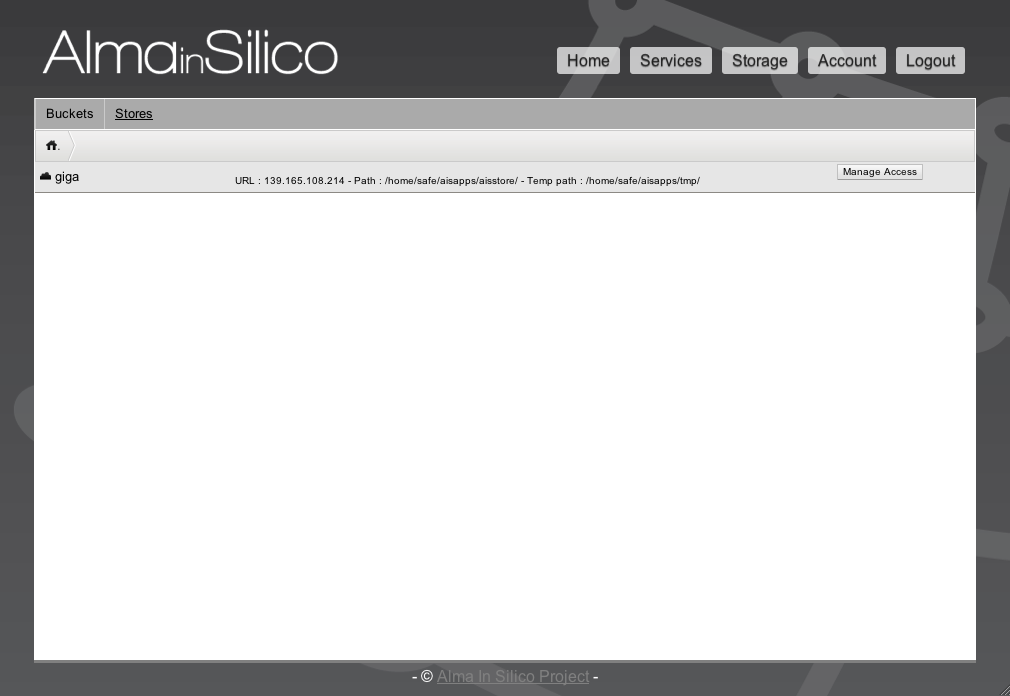
\includegraphics[width=1.0\linewidth]{storesview.png} % requires the graphicx package
   \caption{Store list view.}
   \label{fig:storesview}
\end{figure}

\section{Store creation}
The creation of a \emph{store} is reserved to users with the role allowing them to manage stores. This role can be requested on the account tab on the web application (see figure~\ref{fig:requeststorecreate}. This right is then manually granted by the global administrator. As mentioned in the definition of store, a store is an ssh connection to a file server.
\begin{figure}[htbp]
   \centering
   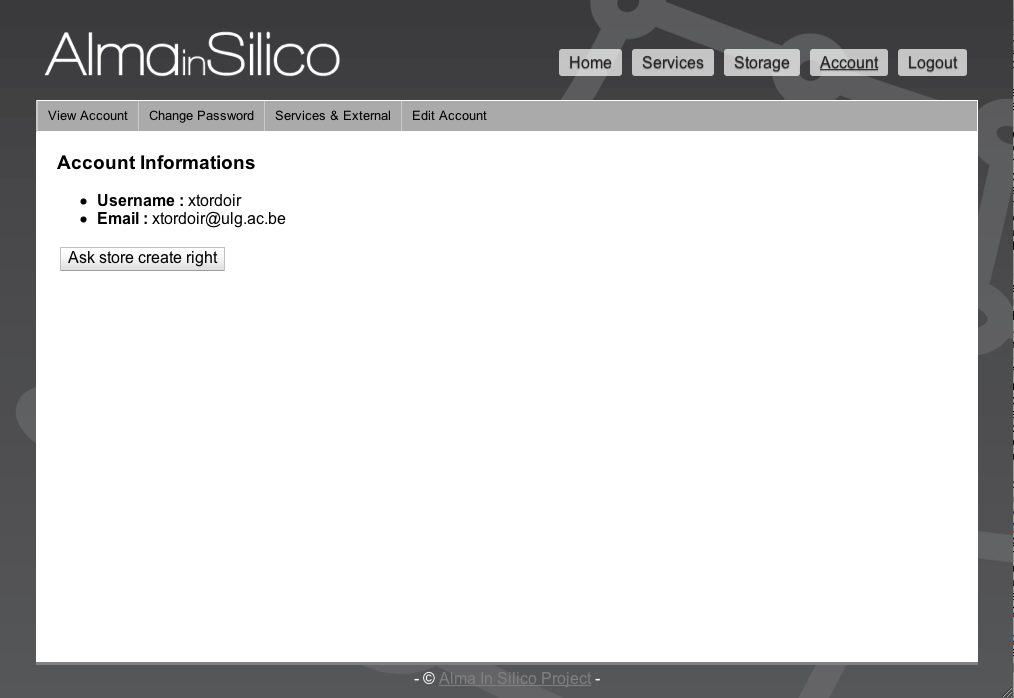
\includegraphics[width=1.0\linewidth]{askstorec.png} % requires the graphicx package
   \caption{Request store creation rights}
   \label{fig:askstorec}
\end{figure}
With this right, a stores can be created.
\subsection{Store definition}
The minimal information required to create a store consists in the following fields:
\begin{itemize}
\item namespace: a unique string identifier for the store, 8 characters maximum, alphanumeric
\item username: the username to be used to login on the remote server
\item store\_url: the server IP or dns
\item path: the absolute path on the server of the data directory
\item tmp: the absolute path on the server of the temporary data, it is used during local copy processes (see ...)
%%\item default: a boolean tag setting the default store %%default is depreciated at this level, default is managed by the global admin
\item description: the text description of the store
\end{itemize}
Store creation is done exclusively on the web application, in the storage tab under the store panel:
\begin{figure}[htbp]
   \centering
   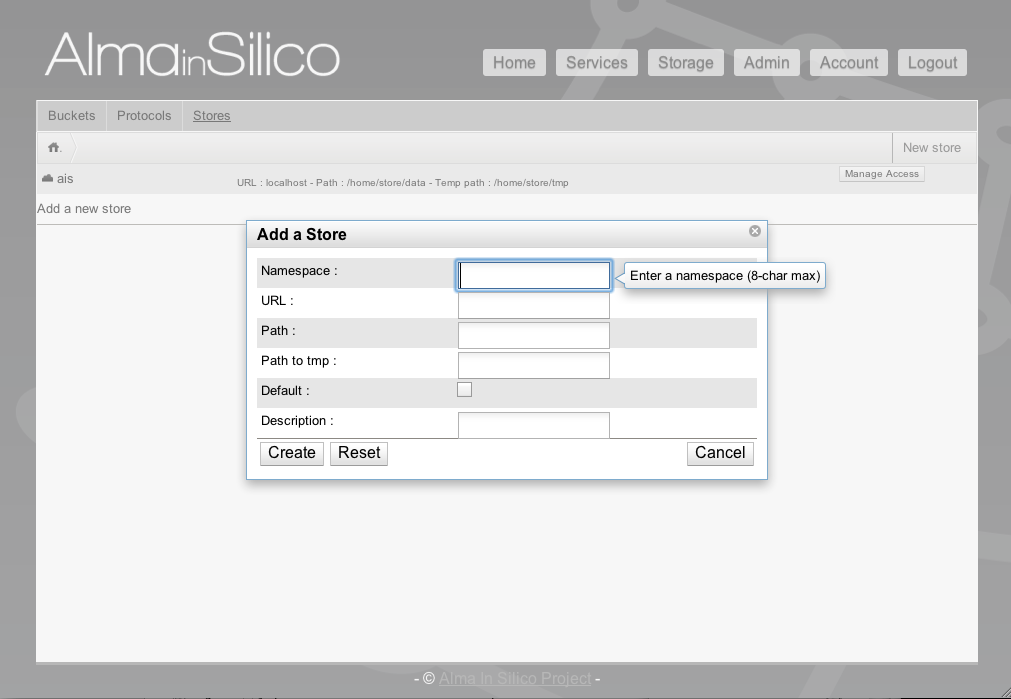
\includegraphics[width=1.0\linewidth]{createstore.png} % requires the graphicx package
   \caption{Store creation form}
   \label{fig:createstore}
\end{figure}
Once a store is created it is not readily available. Of course, the AISStorage web server must be able to access the remote file server. The authentication consists in sharing the ssh public key of the AIS server with the file server.
\subsection{Store validation: AIS public key installation}
For the AIS storage system to work with a store, it must be able to connect to the store. To allow this connection, the store manager must download the AIS rsa public key and install it in its authorized\_keys file. The public key is downloaded from the stores page. The content of this file must be concatenated to the content of the \emph{~/.ssh/authorized\_keys} file on the store.\\
After completion of this operation, the \emph{Put online} button on the store list can be pushed to validate the connection. By this action, the store manager actually asks the AIS server to try to connect to the store and check that the store is correctly configured: it checks if the data and tmp directories exist and have the correct access rights (must be writable) or tries to create them. If these operations are a success, the store is online and can be accessed by users, or put offline. If the store cannot be put online, the manager is notified and can try again after adjusting the store or server configuration.
\begin{figure}[htbp]
   \centering
   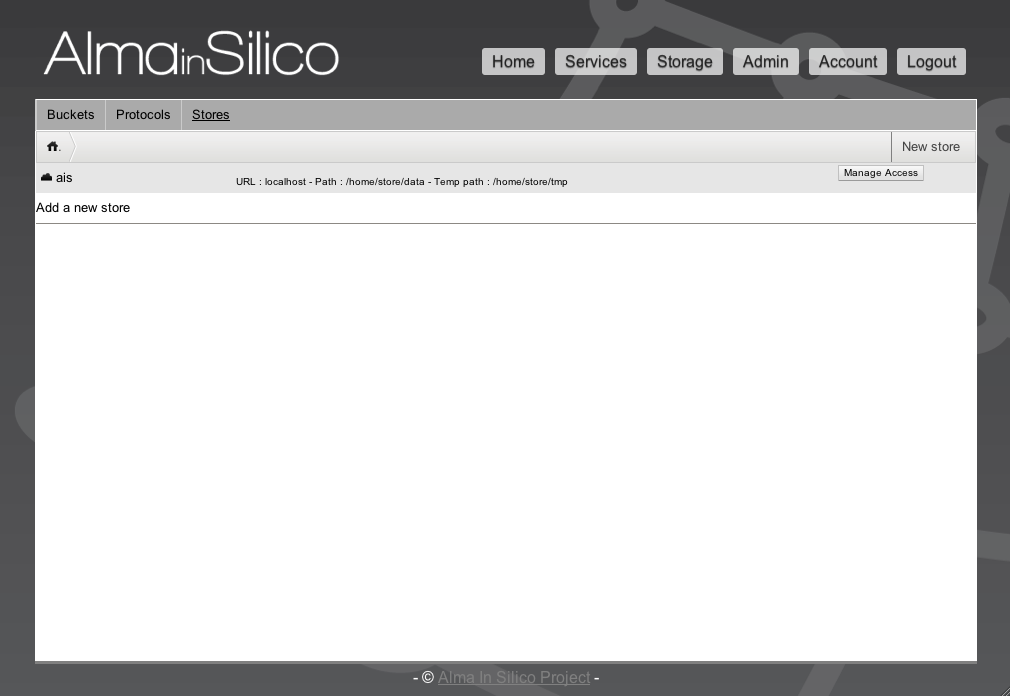
\includegraphics[width=1.0\linewidth]{getkey.png} % requires the graphicx package
   \caption{Download the public key, then put the store online}
   \label{fig:getkey}
\end{figure}

\section{Store rights management}
The creator of a store is granted administration rights and is able to grant rights on the store to other users. Some right can be applied to all users at once, these public rights are:
\begin{itemize}
\item visibility: control whether the store is visible to all users. If yes, all users in the system are aware that the store exists, although they don't have access to the store, they are able to make a request to access it, directly from the store list. The store administrator will accept or reject such requests.
\item writable for all: this controls whether all users have a write access on the store. This only works if the store is visible.
\end{itemize}
The rights granted to users (by email address) are:
\begin{itemize}
\item Admin: read and write access, administration rights (users management)
\item Users: read and write access, can download and upload files on the store
\item viewer: read access, can download files from the store
\end{itemize}
To grant a right to one or several users, email addresses must be entered in the field and validated.
\begin{figure}[htbp]
   \centering
   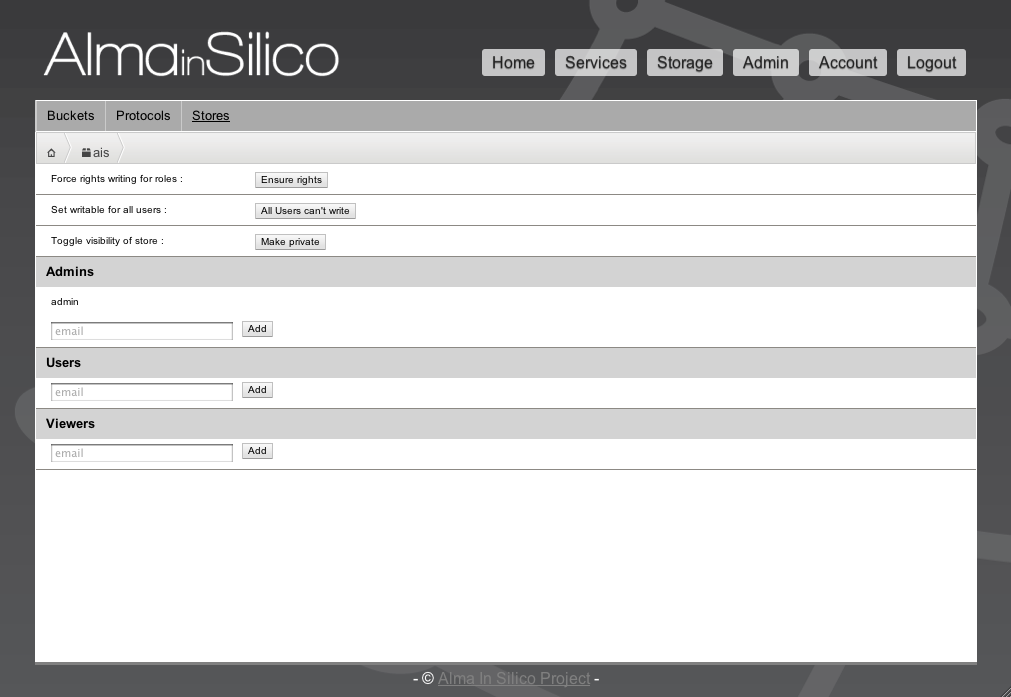
\includegraphics[width=1.0\linewidth]{storeacl.png} % requires the graphicx package
   \caption{Store rights management page}
   \label{fig:storeacl}
\end{figure}
% BUCKET MANAGEMENT
\chapter{Bucket management}
All users have the ability to create and manage their own buckets.
\section{Buckets general navigation}
From the \emph{Storage} tab, the bucket panel is available and features the list of buckets the user has access to. Read only buckets provide a button to request write access, and if administration rights are granted, an access to the rights management page is also available.\\
It is from that view that new buckets can be created as well (see figure~\ref{fig:bucketsview}).
\begin{figure}[htbp]
   \centering
   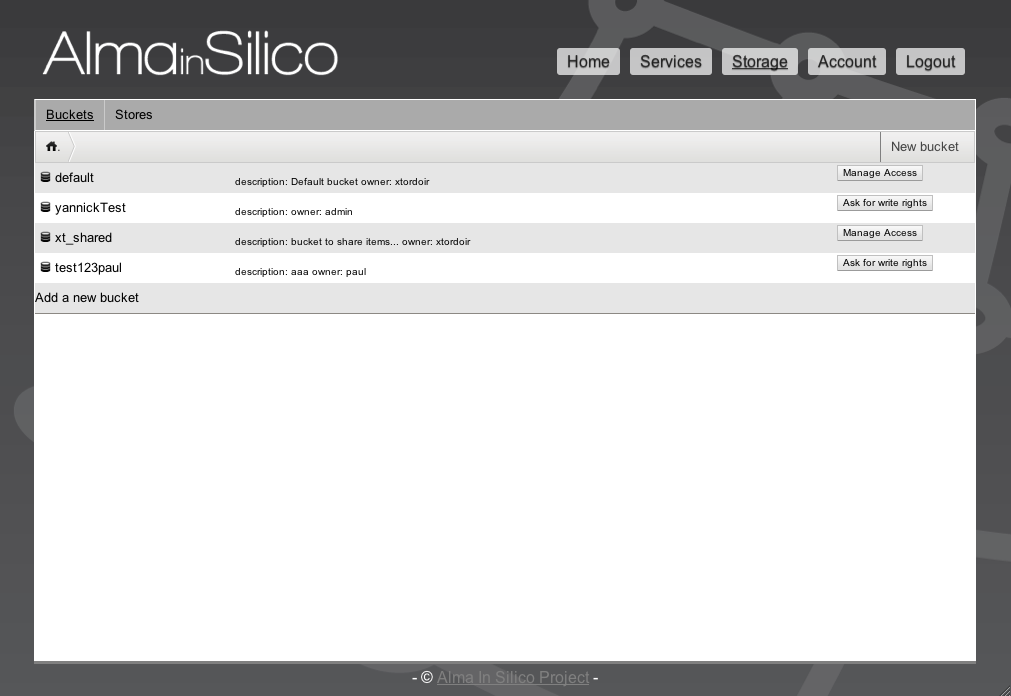
\includegraphics[width=1.0\linewidth]{bucketsview.png} % requires the graphicx package
   \caption{Bucket list view.}
   \label{fig:bucketsview}
\end{figure}

\section{Bucket creation}
\subsection{Bucket definition}
In order to create a bucket, the minimal information required are the following mandatory fields:
\begin{itemize}
\item name: the name of the bucket, unique across all users buckets.
\item description: a text description of the bucket
\end{itemize}
Other available options for advanced configuration can be selected. These control the details on how files are organized on the different stores. As these options cannot be changed, it is important to understand what they mean if default values are not used. It is advisable to have a reason to select non default values:
\begin{itemize}
\item store.multiplicity: the multiplicity of stores used by the bucket, can be \emph{unique} or \emph{multiple}. A multiple store allows to store files on multiple devices, it is the default value. Multiple devices allows to spread the data over different servers, it is meaningful different data are generated "close" to different stores and file transfer shouldn't be performed unnecessarily. A unique store is selected when a tight control on files location must be enforced, and all data should be physically located in a single place, for example close to a data processing facility.
\item store.default: the default store, this option is mandatory if store.multiplicity is \emph{unique}.
\item fs.mapping: the filesystem mapping type, can be either \emph{mirror} or \emph{tree}. The mirror mapping means that object keys are paths on the physical storage. Such a path is relative to the store data directory path. The default is \emph{mirror} as it allows to manage data as in a filesystem. This ensures that all files are at leaves in the path tree and that exporting a bucket on a local filesystem is simple. On the other hand, it is not possible for an object to point to a file from an other bucket, also, a file cannot have child nodes.

\end{itemize}
\begin{figure}[htbp]
   \centering
   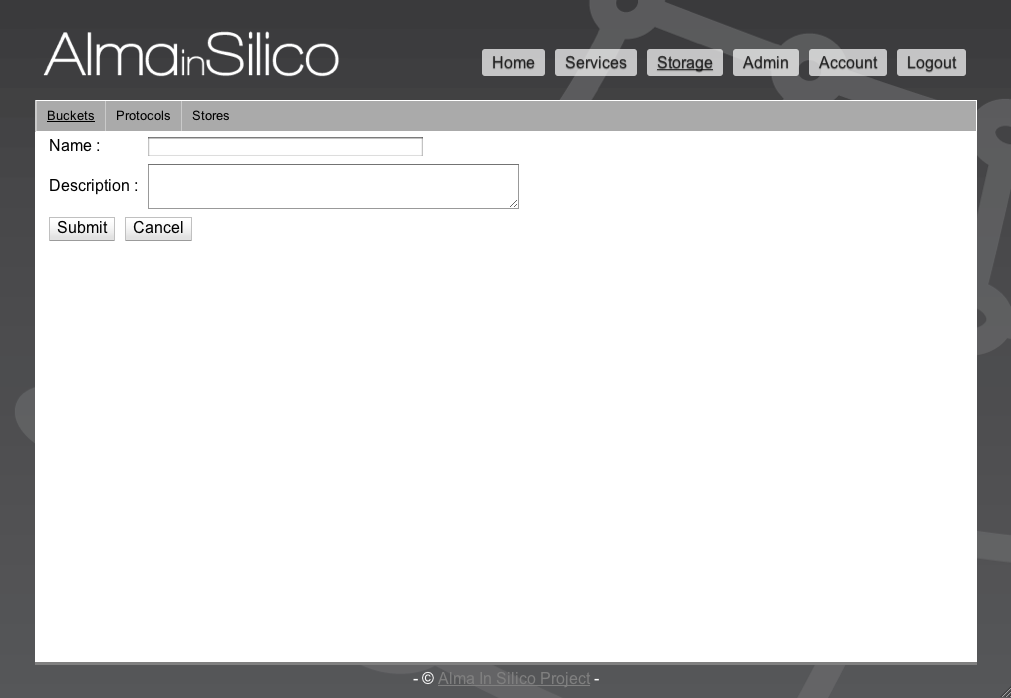
\includegraphics[width=1.0\linewidth]{createbucket.png} % requires the graphicx package
   \caption{Bucket creation form}
   \label{fig:createbucket}
\end{figure}
Once created, the bucket is readily available for use to its creator.
\subsection{Bucket metadata}
While buckets metadata are supported and can be queried and set with the REST API, no view is available from the web UI.
\section{Bucket rights management}
The creator of a bucket is granted administration rights and is able to grant rights on the bucket to other users. A right can be applied to all users at once, this public right is:
\begin{itemize}
\item visibility: control whether the bucket is visible to all users. This allows users to publish data to the public. Also, it provides users with the possibility to request write access to the bucket, this is done directly from the list of buckets. Such a request  will be accepted or rejected by the bucket administrator.
\end{itemize}
The rights granted to users (by email address) are:
\begin{itemize}
\item Admin: read and write access, administration rights (users management)
\item Users: read and write access, can download and upload files on the bucket
\item viewer: read access, can download files from the bucket
\end{itemize}
To grant a right to one or several users, email addresses must be entered in the field and validated.
\begin{figure}[htbp]
   \centering
   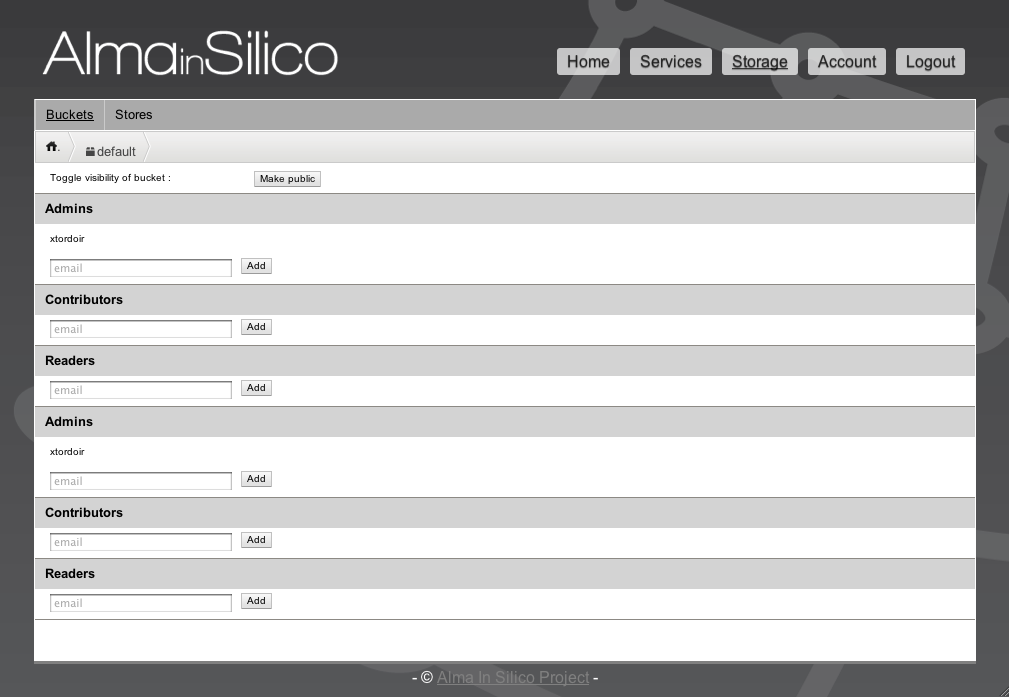
\includegraphics[width=1.0\linewidth]{bucketacl.png} % requires the graphicx package
   \caption{Bucket rights management page}
   \label{fig:bucketacl}
\end{figure}

% OBJECT MANAGEMENT
\chapter{Object management}
From a selected bucket and a given object it is possible to create new objects. From the bucket root, objects can be created in a nested way, and so organized as a tree structure. The '/' characters is used in the object \emph{key} as a separator to jump from one level to the next. The \emph{key} can be seen as a path on the virtual filesystem. For mirrored buckets, the \emph{key} effectively represent a path on the store filesystem. For stores with a \emph{tree} fs.mapping property, there is no guaranteed correspondence between the key and a store filesystem path.\\
As a result, objects can be seen as directories and files.
\section{Object general navigation}
On selection of a bucket, the view shows objects within that bucket and present them as a navigable tree structure. The tree structure is based on the bucket's objects \emph{keys}, using \emph{keys} as if they were paths in the tree using '/' as the separator. Child objects are selected with a simple click and entered with a double click. The navigation bar above the object list is used to return to previous levels.\\
The navigation bar also dispalys the add file and directories buttons.
\section{Object creation: make directory}
The operation of creating a simple object without associated file in a bucket is equivalent to creating a directory. There is no need to create parent directories for this operation to work, and the operation will not create objects for the virtual parent directories. The text representation of the object key is sufficient for the system to understand the implied tree structure.
\subsection{Object definition}
The creation of a simple \emph{object} is reserved to users with write access on the target \emph{bucket}. The fields defining a simple object is:
\begin{itemize}
\item path: the virtual path or \emph{key} of the object. It is a unique identifier also locating the object on the virtual tree structure, using '/' as directory or node separator.
\end{itemize}
\begin{figure}[htbp]
   \centering
   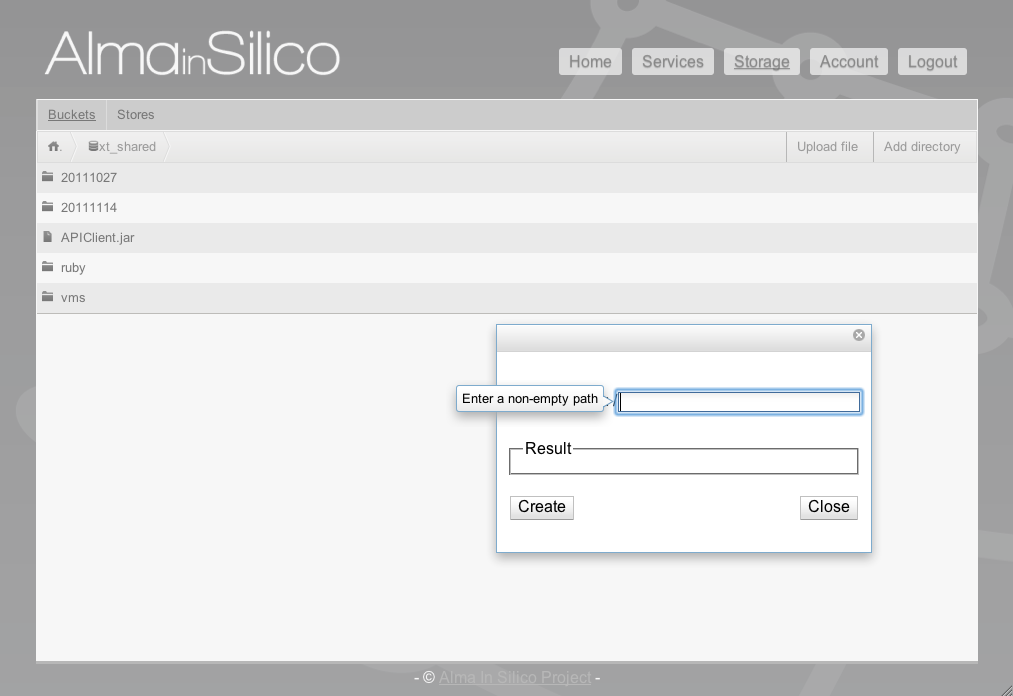
\includegraphics[width=1.0\linewidth]{adddir.png} % requires the graphicx package
   \caption{Object (directory) creation form}
   \label{fig:example}
\end{figure}
\subsection{Object metadata}
The web interface does not allow for the creation or edition of object metadata by the user. The REST API provides this functionality. The only object metadata created from the web interface are the once that identify an object as a file. The object metadata are nevertheless visible.
\subsection{Object creation: upload file}
The operation of putting a file in a bucket consists in creating an object and associating this object with a file on a store. This operation requires to have write access on both the bucket and the store on which the file will be located.
\subsection{Object file definition}
The definition of a file in the AIS storage is actually an extension of the simple object (or directory) definition. For the creation of a file object, the following fields must be filled-in:
\begin{itemize}
\item file: the file path or \emph{key} is constructed from the currently selected object (directory or node) and the filename of the upload item. 
\item \emph{store}: the uploaded file will be stored on a physical device (a store). Only a store for which the user has write permission can be selected.
\end{itemize}
\begin{figure}[htbp]
   \centering
   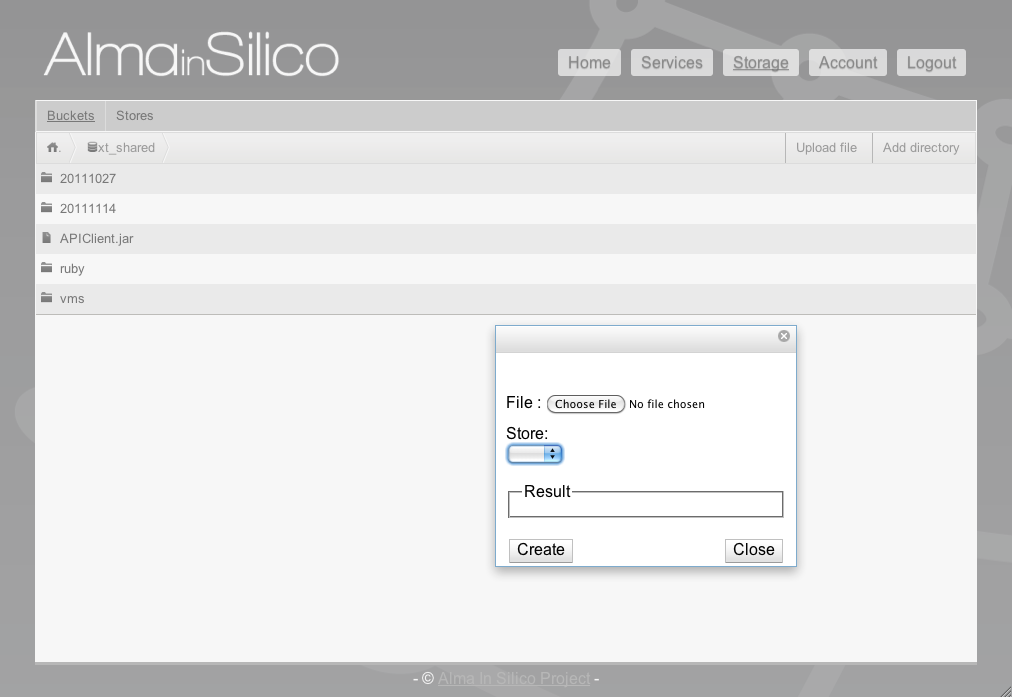
\includegraphics[width=1.0\linewidth]{addfile.png} % requires the graphicx package
   \caption{Object (file upload) creation form}
   \label{fig:example}
\end{figure}
\subsection{Object file metadata}
As mentioned earlier, a file object is an extension of a simple object. The extension is made through the use of object metadata, specific for the file object definition. The set of mandatory metadata required to make an object a file object are the following:
\begin{itemize}
\item url: a string pointing to the physical location of the file. It consists in the \emph{store} and the path on the store relative to the store's data directory.
\item size: the size of the fiel in bytes
\item md5: the md5 of the file
\item username: the username of the user who created the file in AIS storage. The owner of the file is the person responsible for the storage provider's storage usage.
\end{itemize}
All these fields are set automatically by the server during the file upload operation.
\begin{figure}[htbp]
   \centering
   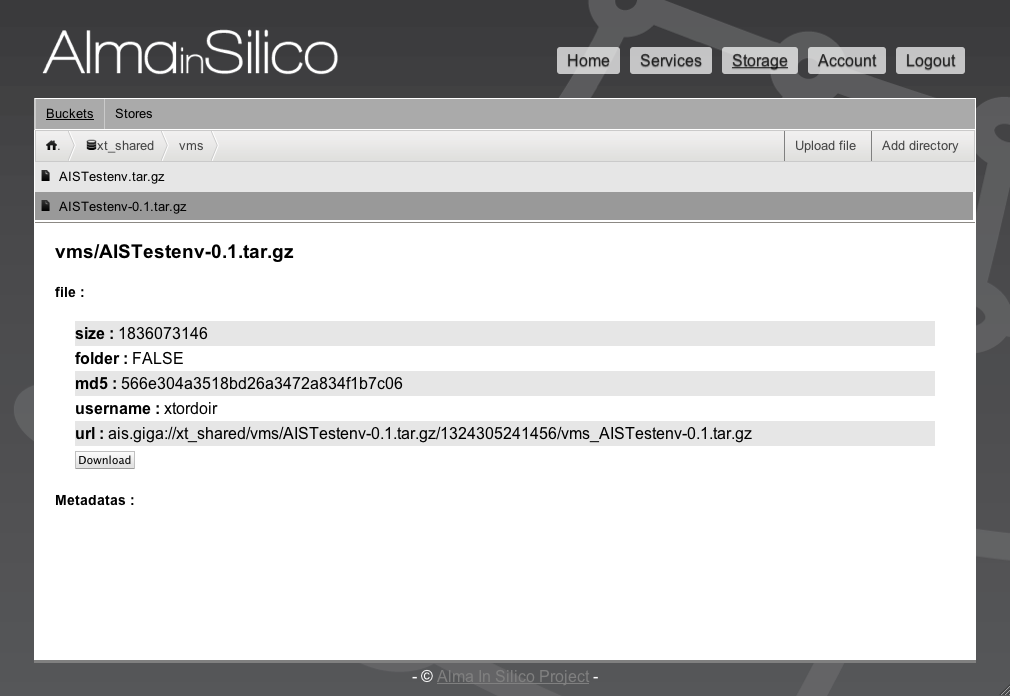
\includegraphics[width=1.0\linewidth]{metaview.png} % requires the graphicx package
   \caption{File object metadata view}
   \label{fig:example}
\end{figure}
\section{Relationship between store and bucket rights}
While the user would like to control access rights on a bucket by just setting the bucket rights management, the combination of store rights and bucket configuration can result in side effect for the bucket rights and the possible operations on objects and associated files.\\
The rule is that always the store rights have precedence over the bucket rights, and store rights only applies to files. For example, if a user has read access on a bucket, he will be able to see the complete list of file even if they are stored on stores he has no read access to. The limitation in this case is that the user is not able to download the file as he has no read access on the store. The same applies for write access. If a user has write access on a bucket configured to work with a unique store for which no write access is granted, the user will not be able to upload files, while he will be able to create objects.

\part{User guide: REST API}
\chapter{Store}
\emph{Stores} cannot be managed with the API, only the web interface allows to create and manage access control on stores.
\chapter{Bucket} 
\section{Bucket creation}
\section{Bucket }
\subsection{Object as File}
\subsection{Object metadata}
\section{Object API}


\end{document}  